\subsection{扰动规模扫描}
\label{sec:scale}

表~\ref{tab:scale} 与图~\ref{fig:scale} 报告 \(\varphi\) 扫描
（\texttt{congested\_8x4x4}, \(\NSeeds\) 个随机种子；R0+ 预算 \(2\)\,s）。
逐档结果见表；\(C_{\max}\) 仍全由 R0+ 更优，与第~\ref{sec:e5}~节一致。
小例 \texttt{example\_3x3x2} 上同样每格可行（\(\NSeeds\) 个随机种子 \(\times\) 五个
\(\varphi\) 值），有界修复约 \(1\)\,ms 量级，
耗时比 \(\SpeedLo\times\)--\(\SpeedHi\times\)（跨两个算例的逐格极值）。该比值以 R0+ 的\emph{预算}为分子、有界修复的实测挂钟为分母，而 R0+ 在 \(C_{\max}\) 上更优，
故不应理解为同等质量下的加速比。

本节的有界修复启用了失败后扩大范围，故结果与 E3、E5 不可直接比较。
即使扰动比例升至 \(\varphi=1\)（全部未来工序受扰动），算法耗时仍在十毫秒量级，不随扰动规模显著增长；
这一耗时来自单遍改路（第~\ref{sec:cheap}~节）。

\begin{table}[t]
\centering
\caption{扰动规模对照（\texttt{congested\_8x4x4}, \(\NSeeds\) 个随机种子平均）。
有界修复含扩大范围；R0+ 预算 \(2\)\,s。离散度按四分位距报告：STRC 耗时全扫描极差为
\ScaleMsMin--\ScaleMsMax\,ms,R0+ \(C_{\max}\) 的逐档 IQR 在 \ScaleCmaxIqrLo--\ScaleCmaxIqrHi
之间。\textbf{「耗时比」一列在最小两档上的档内 IQR 已超过该列的档间起落，
故它只反映量级，不指示随 \(\varphi\) 变化的趋势。}该列为\emph{逐格}比值的档均值（先配对、后统计），
因此不等于相邻两列档均值之比；由 \(1/x\) 的凸性，两者一般不同，复算时应使用逐格数据。
分子是 R0+ 的挂钟\emph{预算}而非其实测耗时，故这不是同质量下的比较（第~\ref{sec:protocol}~节）。}
\label{tab:scale}
\small
\begin{tabular}{@{}rcccc@{}}
\toprule
\(\varphi\) & STRC 可行 & STRC\,ms & R0+ \(C_{\max}\) & 耗时比 \\
\midrule
\(0.10\) & \(100\%\) & \(9.1\)  & \(103.5\) & \(406\times\) \\
\(0.25\) & \(100\%\) & \(11.1\) & \(107.0\) & \(325\times\) \\
\(0.50\) & \(100\%\) & \(8.6\)  & \(111.8\) & \(333\times\) \\
\(0.75\) & \(100\%\) & \(8.4\)  & \(125.8\) & \(254\times\) \\
\(1.00\) & \(100\%\) & \(10.7\) & \(148.1\) & \(203\times\) \\
\bottomrule
\end{tabular}
\end{table}

\begin{figure}[t]
\centering
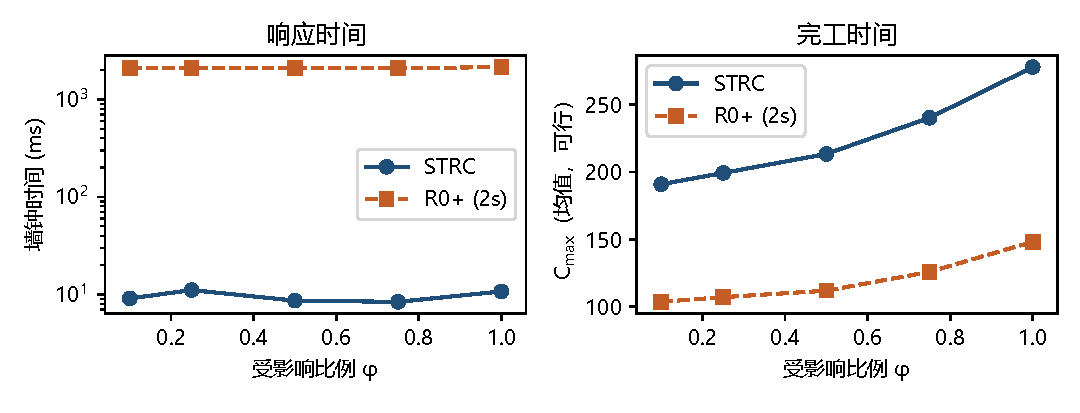
\includegraphics[width=\linewidth]{figures/fig_strc_scale_CN}
\caption{扰动规模扫描（\texttt{congested\_8x4x4}, \(\NSeeds\) 个随机种子）：
有界修复与 R0+ 的算法耗时（对数轴）与完工时间随 \(\varphi\) 变化。曲线取逐档均值，
离散度口径与表~\ref{tab:scale} 同（四分位距）；耗时一侧全扫描极差
\ScaleMsMin--\ScaleMsMax\,ms，始终在十毫秒量级，这是本节结论所依据的唯一结果。}
\Description{两条随扰动比例变化的曲线。算法耗时画在对数纵轴上：有界修复始终在
十毫秒量级、不随比例上升而显著增长，全局重调度固定在两秒的预算线上。完工时间一侧，
全局重调度随扰动比例增大而缓慢上升，但始终低于有界修复。}
\label{fig:scale}
\end{figure}

\subsection{E8：算例规模上的外推}
\label{sec:instscale}

上一节扫描的是\emph{扰动}的规模，算例始终为 \(8\) 工件 \(4\) 机。本节转向另一维：固定扰动协议，
扩大算例本身。此处的关键不在耗时（耗时不显著增长是可以预期的），而在于\textbf{影响集占比是否会
随规模增大而接近 \(1\)，使「有界」失去实际意义}。

规模序列取工件数 \(2k\)、机器数 \(k\)、车辆数 \(k\),\(k=4,\dots,10\)，即 \(8\times4\times4\) 到
\(\ScaleJobsHi\times\ScaleMachHi\times\ScaleMachHi\)，共 \(\ScaleKs\) 档 \(\times\)
\(\NSeeds\) 个随机种子 \(=\ScalePairs\) 对。拥堵档、异构度、柔性度、运输/加工时长比与装卸站
最小割、远端割全部按同一目标标定，\emph{只改变规模}。三个对照方法与第~\ref{sec:cheap}~节定义相同。

\begin{table}[t]
\centering
\caption{E8 算例规模扫描（\(\ScaleKs\) 档 \(\times\) \(\NSeeds\) 个随机种子）。
「影响集」为预约影响集占\emph{全表}之比，该比的可达上界是 \(|R^{\circ}|/|R|\)、本批均值约
\ScaleAliveShare；换以可改写集合为分母则为 \ScaleCloAliveLo--\ScaleCloAliveHi（见正文）。
耗时取中位数，「RD/R2」一列即两列\emph{中位数之比}；正文讨论其单调性时用的是逐格配对后的
档均值，两种口径的档间起落一致但数值不同。末列为 R2 对 RS 的 \(C_{\max}\) 胜负。}
\label{tab:instscale}
\small
\begin{tabular}{@{}lrccccc@{}}
\toprule
规模 & \(|R|\) & 影响集 & R2\,ms & RD\,ms & RD/R2 & R2 对 RS \\
\midrule
\(8\times4\times4\)    & \(148\) & \(0.561\) & \(2.9\)  & \(4.4\)  & \(1.5\times\) & \(7/1/2\) \\
\(10\times5\times5\)   & \(172\) & \(0.485\) & \(3.2\)  & \(6.1\)  & \(1.9\times\) & \(9/0/1\) \\
\(12\times6\times6\)   & \(230\) & \(0.481\) & \(4.5\)  & \(10.7\) & \(2.4\times\) & \(7/1/2\) \\
\(14\times7\times7\)   & \(281\) & \(0.492\) & \(6.1\)  & \(14.5\) & \(2.4\times\) & \(8/0/2\) \\
\(16\times8\times8\)   & \(291\) & \(0.534\) & \(6.4\)  & \(16.4\) & \(2.6\times\) & \(10/0/0\) \\
\(18\times9\times9\)   & \(356\) & \(0.535\) & \(8.2\)  & \(26.4\) & \(3.2\times\) & \(10/0/0\) \\
\(20\times10\times10\) & \(402\) & \(0.476\) & \(10.4\) & \(34.2\) & \(3.3\times\) & \(10/0/0\) \\
\bottomrule
\end{tabular}
\end{table}

逐档结果见表~\ref{tab:instscale}。

\textbf{影响集占比不随规模增大而上升，但「是否接近 \(1\)」须换用恰当的分母才能回答。}
七档 \(\mathrm{Cl}/|R|\) 在 \ScaleCloLo--\ScaleCloHi 之间波动，且不单调
（首档最高、末档最低，第五、六两档回到 \(0.53\) 以上）。由于 \(\mathrm{Cl}\) 只包含
\(t_{\mathrm{now}}\) 之后尚未结束的占用，而本批 \(|R^{\circ}|/|R|\) 均值仅为 \ScaleAliveShare，
\(\mathrm{Cl}/|R|\) 的可达上界约为 \ScaleAliveShare 而非 \(1\)。以可改写集合为分母时，
七档 \(\mathrm{Cl}/|R^{\circ}|\) 落在 \ScaleCloAliveLo--\ScaleCloAliveHi（逐格最高为 \(1.00\)），
与第~\ref{sec:e6}、\ref{sec:cheap}~两节主批次的 \ClosureAliveFrac\ 同量级。
因此本节表明\emph{占比不随规模增大而上升}，但影响集相对可改写集合并不小（注~\ref{rem:minimality}）；
七档数据也不足以支持渐近结论。

\textbf{算法耗时的增长快于占用总数的增长。} \(|R|\) 增至 \(2.7\) 倍时，R2 的耗时中位数从
\(2.9\)\,ms 增至 \ScaleMsHi\,ms，即 \(3.6\) 倍，仍在十毫秒量级；七档数据不足以确定增长阶。第 1 级改路的可行格数为 \ScaleFeasFirst；
唯一失败的一格（\(10\times5\times5\)，随机种子 \(42\)）经失败后扩大范围在第 \(3\) 轮恢复可行，
总耗时 \(12.0\)\,ms，完工时间与第 1 级尝试相同，故最终可行格数为 \ScaleFeasAll。

\textbf{两种对照方法的耗时差距随规模增大。} 耗时最短的全局重算与有界修复的耗时比
从 \ScaleRatioLo\(\times\) 升至 \ScaleRatioHi\(\times\)，即规模越大，全局重算的耗时代价越高。
逐档比值\emph{并不单调}（逐格配对后的档均值在 \(k=6\to 7\) 处回落），但两端相差 \(1.8\)，
远大于任一档内不超过 \(0.74\) 的四分位距，故\emph{总体上升}并非噪声。

与不按影响集划界的全局右移相比，R2 的 \(C_{\max}\) 胜负在最后三档均为 \(10/0/0\)，前四档则在
\(7\)--\(9\) 胜之间，无单调变化；每档只有 \NSeeds\ 格，不足以判断趋势。

\textbf{口径限制。} 这一规模序列只有一个拥堵档和一个算例随机种子（每档的算例均由随机种子
\(42\) 生成），只检验\emph{规模}这一维；第~\ref{sec:e6}、\ref{sec:scale}~两节的扫描未在这批算例上重新运行。
就贡献而言，本节为 C2 的有界性补充了规模方向的证据：占比在这七档上没有上升。

\subsection{外部布局批次的复现}
\label{sec:pubrepro}

第~\ref{sec:protocol}~节第二批把布局出处换成外部来源后，\(\NPubPairs\) 个算例--随机种子对上
E1、E2、E3、E5 的结果与主批次\emph{逐项同向}：
工序依赖图给出空范围 \PubPassMiss，结构包含性（即泄漏计 \(0\)）\PubPassClosed，
集外字段逐条不变 \PubPassInvar；边界消融下第 1 级改路的可行格数为 \PubFeasRone，
按预约影响集划界为 \PubFeasRtwo。E1 协议下影响集占比的逐布局中位数落在
\PubEoneFracLo--\PubEoneFracHi；同口径的主批次结果是 \NPairs\ 对合并后的中位数 \EoneFracMed
（\EoneCloLo--\EoneCloHi\ 是逐算例\emph{均值}的极差，口径不同）。
外部批次整体略低，但两者均约为一半，且偏低幅度与算例间差异同量级（第~\ref{sec:e1}~节图注）。
与全局重调度的权衡亦无变化：\PubEfiveNoCross\ 个预算点上 R0+ 的 \(C_{\max}\) 更优，
余下 \(1\) 点两法持平（\texttt{LyuL6\_8m}，随机种子 \(2024\)，预算 \(0.2\)\,s），无一点更差。
这批与主批次使用同一份 E5 代码和同一组参数，故第~\ref{sec:e5}~节按 \(\EfiveCells\) 个
算例--随机种子格合并分析两批；持平的一格同样满足该节的单调性判断，交叉点仍不存在。

这一批用于检验上述现象是否只在本文设计的布局上成立：结果在一批并非由本文选定的拓扑上同样成立，
故 C1 与 C2 的对象层不依赖本文的布局设计。这批算例唯一改变的是结构可预测性的结论（第~\ref{sec:e4}~节）。

\subsection{小结}
\label{sec:exp_summary}

本章结果按其支撑的贡献层归并；各项局限及其影响的层次集中见第~\ref{sec:limitations}~节。

\textbf{对象层}（C1、C2：按什么对象划界、划出的集合是否唯一确定）由四组结果支撑。
走廊阻断下工序依赖图上的范围为空，而原排程确已不可行（E1,\(\NPairs\) 对上 \(\PassMiss\)）；
预约影响集对依赖边封闭，集外字段逐条不变(E2,\(\PassClosed\)、\(\PassInvar\))；
同一套改路程序只更换划界对象，恢复可行率即由 \(\FeasRone\) 变为 \(\FeasRtwo\)(E3)，
因此可行与否取决于划界对象，而非改路程序的优劣；在四类扰动与两种划界对象的交叉中 A/B 二分无例外，
且 A 类上预约影响集均包含工序依赖图划界的结果(E6)。
命题~\ref{prop:miss}--\ref{prop:outside} 给出对应的结构陈述，
其中命题~\ref{prop:outside} 仍只作充分条件。

\textbf{净收益层}（C3：这样划界带来什么收益）只由一组结果支撑：换用不按影响集限制范围的对照
（RA，与 R2 使用同一套改路，同样不改写已经结束的占用）后，算法耗时与 \(C_{\max}\) 几乎不变，
改动比例却由 \ResFracCheapRtwo\ 升至 \ResFracAllFuture（逐格 \RAStabWTL,\(p=\RAStabP\)；
第~\ref{sec:cheap}~节）。故毫秒量级的响应来自单遍改路而非影响集，
\textbf{改写量的减少只能由这一对照得出}。与热启动全局重调度相比，有界修复在 \(C_{\max}\) 上
无一格更优，放宽预算也不出现反超(E5);E7 则排除了「对照方法耗时过长」这一解释。

其余结果为限定性结果：算例规模已扩展至 \(\ScaleJobsHi\) 工件
\(\ScaleMachHi\) 机，以可改写集合为分母的影响集占比未随规模上升(E8)；
结构可预测性是负结果(E4)。第二批算例（\(\NPubPairs\) 对）只检验上述现象是否依赖
本文自行设计的布局，E1、E2、E3、E5 的结果逐项复现。

%% =====================================================================
\section{总结}
\label{sec:conclusion}
%% =====================================================================

本文有三项贡献。\textbf{其一}(C1)，指出了一类工序依赖图无法刻画的失效：走廊阻断不改变任何工序指派，
按受影响工序划出的范围为空，而原排程确已不可行（\(\NPairs\) 对上 \(\PassMiss\)，第~\ref{sec:e1}~节）。
\textbf{其二}(C2)，以 \STRC 得到的预约影响集作为重调度范围：依赖关系一经给定，一条占用是否属于该集合即
唯一确定，集内没有指向集外的依赖边（\(\PassClosed\)、\(\PassInvar\)，第~\ref{sec:e2}~节）。
\textbf{其三}(C3)，给出与该划界相匹配的局部恢复，并区分各项结果的来源：同一套改路程序只更换划界对象，
恢复可行率即由 \(\FeasRone\) 变为 \(\FeasRtwo\)（第~\ref{sec:e3}~节），
因此可行与否取决于划界对象，而非改路程序的优劣。

让行关系、集内改路而集外保持原计划、失败后扩大允许改写的范围均沿用既有文献
（第~\ref{sec:rw_claim}~节）。本文的主张是：
工序依赖图按定义不含走廊占用之间的让行关系，因而无法刻画只使占用失效的扰动；
在预约依赖图上划界后，须改写的占用由既定先后关系唯一确定，而非取决于启发式半径。

将允许改写的集合从预约影响集换为「\(t_{\mathrm{now}}\) 之后尚未结束的全部占用」、
其余条件不变时，算法耗时与完工时间几乎不变，改动比例却由 \ResFracCheapRtwo\ 升至
\ResFracAllFuture（第~\ref{sec:cheap}~节）。
故毫秒量级的响应来自单遍改路、不重新启动搜索；\textbf{改写量的减少只能由这一对照得出，
它体现的是命题~\ref{prop:outside} 所保证的性质：集外占用保持原计划}。
收益幅度取决于影响集比该平凡上界小多少，两者接近时收益趋于消失。

\subsection{局限}
\label{sec:limitations}

以下四条按对前文结果的影响排序，第~\ref{sec:future}~节逐条给出推进方向。

\begin{enumerate}[leftmargin=1.6em,itemsep=0.35em]
\item \textbf{完工时间劣于不改写已结束占用的热启动全局重调度，且放宽预算不出现反超。}
有界修复以完工时间换取算法耗时，而这一劣势在所测的 \(\EfiveCells\) 个算例--随机种子格上
不随预算放宽而反转（第~\ref{sec:e5}~节）。
该局限关系到划界的净收益，而不涉及对象层的结论；改写量的比较见第~\ref{sec:cheap}~节。

\item \textbf{对预约影响集，命题~\ref{prop:outside} 的保证只是充分条件，依赖边集未经独立的
穷尽检验，允许改写的集合不紧，其规模也不能由仅依赖路网的静态指标预测。}
影响集覆盖 \(t_{\mathrm{now}}\) 之后尚未结束占用的约 \(\ClosureAliveFrac\)（注~\ref{rem:minimality}），
净收益的幅度取决于影响集小于该平凡上界的程度，两者接近时收益趋于消失。
静态割这一族指标已由第~\ref{sec:e4}~节排除，路网几何与影响集规模的一般关系仍待研究。
该局限关系到对象层保证的强度与紧度，不影响「按工序依赖图划界会给出空范围」这一诊断。

\item \textbf{实现覆盖小于正文所述的问题范围：B 类扰动仅以改路响应，A 类另允许换车与改派
但不改变加工顺序，且由假设 A3 只做一次响应。}
放开加工顺序即向全局重调度退化，「有界」随之失去意义；扰动流、预测误差与滚动响应均未涉及。
规模一维已扩展至 \(\ScaleJobsHi\) 工件 \(\ScaleMachHi\) 机且影响集占比未随规模上升，
但所扫档数不足以支撑渐近论断。该局限限制了结果向更大规模与连续扰动的外推。

\item \textbf{外部参照缺位：这一类研究没有可换用的公开基准，算例出处只外部化到拓扑一层，
结果亦未在第二套实现上复现。}
公开算例族~\cite{homayouni2021production,bilge1995time} 把运输时间发布为机器间行程时间矩阵而不是路网，两族共 \(11\) 张布局逐张检验没有一张
能还原成与所发布矩阵一致的无向走廊图，\(R\)、\(G_R\)、\(\mathrm{Cl}(\cdot)\) 与 B 类扰动
在其上均无法定义（第~\ref{sec:protocol}~节）。
第二批算例按 Lyu 等~\cite{lyu2019approach} 的附录布局构造，布局因此不再由本文设计，
但逐段行驶时间与工件数据仍出自本文，故不能用来复现 Lyu 或 van Os~\cite{vanos2026exact} 的参照值，
其覆盖范围也小于主批次。该局限关系到外部效度，同一实现内各对照之间的相对结果不受影响。
\end{enumerate}

\subsection{后续工作}
\label{sec:future}

下列四条与上一节的四个局限一一对应。

\textbf{一、缩小完工时间上的差距}（局限 \(1\)）。
在主批次中，前缀解码不改写已结束的占用（E5 的 \(18\) 个预算点越界数为 \(\RzeroPastLo\),
E7 上 RD 为 \RedecodeBad），故局限 1 仅涉及 \(C_{\max}\) 本身。
若要缩小差距，须在不改写已结束占用的前提下进行有限度的改派或改序，但这会使方法向全局重调度退化。

\textbf{二、使预约影响集的保证更完备、更紧，并刻画其规模}（局限 \(2\)）。
\emph{完备性}：在当前让行边集下，试探泄漏为 \ProbeLeaks；
下一步是采用其他扰动形态（例如缩短占用，或延后超过 \(1\) 个时间单位）进行试探，而非继续补充同类依赖边。
\emph{紧度}指向最小允许改写集合：在固定修复能力下定义最小性，
并给出影响集与之的差距，这是把「有界」从充分条件推进到紧界的必要步骤；当前影响集覆盖约
\(\ClosureAliveFrac\) 的尚未结束占用，两者的差距可能相当大。\emph{规模刻画}目前只有一条
事后规则（允许改写占比，图~\ref{fig:worth}），但它随排程而变，须改用可在扰动前计算的指标。
第~\ref{sec:e4}~节已排除静态割这一族指标：它在实际布局上取值恒定，而同一张路网上
仅改变机器配置，影响集占比即发生变化，\(4\times 4\) 路网上由 \(4\) 机改为 \(5\) 机即变化 \PubCloSpread,
\(5\times 5\) 路网上改变三种配置（\(6\)、\(7\)、\(8\) 机）变化 \PubCloSpreadBig。
这提示起作用的可能是\emph{需求的空间分布}，而非路网所提供的通行能力。
下一个候选是 \(t_{\mathrm{now}}\) 邻域内的走廊占用时序密度，例如受扰走廊在其繁忙窗口内的
重叠占用条数、以及该走廊在让行图上的出度。这类量随排程而变，不再是纯拓扑量，
「可预测性」的提法也须随之改为给定布局\emph{与当前排程}预测规模。

\textbf{三、放开假设 A3}（局限 \(3\);A3 为单次、完全观测）。
下一步不在于进一步开放改序，而在于放开该假设，考察影响集在连续扰动下是否会累积膨胀，
以及两次修复之间是否需要显式的「归位」步骤。

\textbf{四、使时间标定同样采用外部来源}（局限 \(4\)）。布局已采用外部来源；时间标定方面，
仍需一份同时发布\emph{排他路网与逐段时长}的算例族，自建边权扫描不能替代。
第二套独立实现无须单独开展，可在复现上述任一项时一并完成。

%% 规范项收口:基金、致谢、利益冲突三项按期刊通例齐备。
%% acmart 的 acks 环境在 review/anonymous 模式下自动隐去,故匿名投稿无需手工删。
\begin{acks}
本文工作由 <待填：基金项目名称与编号> 资助。
作者感谢匿名审稿人对实验口径与结论边界提出的意见。
\end{acks}

\section*{利益冲突声明}
作者声明不存在与本文工作相关的利益冲突。

\bibliographystyle{ACM-Reference-Format}
\bibliography{reference-base}

\end{document}
